% Tool-demo paper (candidate: a 4-page ACM tool-demo track, e.g. FSE or ASE Tool Demos). Venue not final.
% Every number comes from ../generated/numbers.tex.
\documentclass[sigconf]{acmart}
\usepackage{booktabs,xspace}
% generated by scripts/make_paper_numbers.py
\newcommand{\nCorpus}{54{,}058\xspace}
\newcommand{\nAnchored}{51{,}697\xspace}
\newcommand{\nUnres}{2{,}361\xspace}
\newcommand{\pctUnres}{4.4\xspace}
\newcommand{\pctReach}{56.6\xspace}
\newcommand{\ciReach}{[56.2, 57.1]\xspace}
\newcommand{\ciReachRepo}{[53.9, 59.3]\xspace}
\newcommand{\pctReachHigh}{44.8\xspace}
\newcommand{\ciReachHigh}{[44.4, 45.3]\xspace}
\newcommand{\meanReach}{18.8\xspace}
\newcommand{\ciMeanReach}{[18.6, 19.1]\xspace}
\newcommand{\medianReach}{1.3\xspace}
\newcommand{\nRepos}{8{,}548\xspace}
\newcommand{\nTyped}{2{,}630\xspace}
\newcommand{\catUnrel}{42.9\xspace}
\newcommand{\catDocs}{22.6\xspace}
\newcommand{\catTests}{15.7\xspace}
\newcommand{\catFmt}{12.6\xspace}
\newcommand{\catDeps}{7.8\xspace}
\newcommand{\catCI}{5.8\xspace}
\newcommand{\reachClaude}{52.6\xspace}
\newcommand{\stdClaude}{55.9\xspace}
\newcommand{\filesClaude}{4\xspace}
\newcommand{\bigClaude}{16.8\xspace}
\newcommand{\reachCopilot}{82.3\xspace}
\newcommand{\stdCopilot}{62.9\xspace}
\newcommand{\filesCopilot}{15\xspace}
\newcommand{\bigCopilot}{46.3\xspace}
\newcommand{\reachCodex}{56.4\xspace}
\newcommand{\stdCodex}{58.3\xspace}
\newcommand{\filesCodex}{4\xspace}
\newcommand{\bigCodex}{16.2\xspace}
\newcommand{\reachCursor}{67.6\xspace}
\newcommand{\stdCursor}{66.5\xspace}
\newcommand{\filesCursor}{5\xspace}
\newcommand{\bigCursor}{19.3\xspace}
\newcommand{\reachDevin}{49.9\xspace}
\newcommand{\stdDevin}{57.0\xspace}
\newcommand{\filesDevin}{3\xspace}
\newcommand{\bigDevin}{12.6\xspace}
\newcommand{\reachJules}{40.4\xspace}
\newcommand{\stdJules}{57.9\xspace}
\newcommand{\filesJules}{2\xspace}
\newcommand{\bigJules}{11.0\xspace}
\newcommand{\missCopilot}{1.2\xspace}
\newcommand{\missAll}{1.3\xspace}
\newcommand{\noncodeCopilot}{11.7\xspace}
\newcommand{\noncodeAll}{19.5\xspace}
\newcommand{\readmeCopilot}{11.4\xspace}
\newcommand{\readmeOther}{6.6\xspace}
\newcommand{\instrCopilot}{5.0\xspace}
\newcommand{\instrOther}{0.1\xspace}
\newcommand{\pkgCopilot}{7.9\xspace}
\newcommand{\pkgOther}{3.3\xspace}
\newcommand{\mergedReach}{57.9\xspace}
\newcommand{\unmergedReach}{54.1\xspace}
\newcommand{\mergeRaw}{+3.8\xspace}
\newcommand{\mergeStd}{-0.5\xspace}
\newcommand{\ciMergeStd}{[-4.5, 2.9]\xspace}
\newcommand{\taskFeat}{84.8\xspace}
\newcommand{\taskNFeat}{1{,}087\xspace}
\newcommand{\taskFix}{63.7\xspace}
\newcommand{\taskNFix}{1{,}022\xspace}
\newcommand{\taskRefactor}{82.3\xspace}
\newcommand{\taskNRefactor}{169\xspace}
\newcommand{\taskDocsTask}{66.2\xspace}
\newcommand{\taskNDocsTask}{162\xspace}
\newcommand{\unresDocsTask}{19.8\xspace}
\newcommand{\nPai}{3{,}087\xspace}
\newcommand{\nPaiSC}{455\xspace}
\newcommand{\nPaiUnres}{21\xspace}
\newcommand{\nPaiBench}{500\xspace}
\newcommand{\nPaiGym}{2{,}287\xspace}
\newcommand{\nPaiML}{300\xspace}
\newcommand{\aucFence}{0.577\xspace}
\newcommand{\ciAucFence}{[0.554, 0.601]\xspace}
\newcommand{\aucSize}{0.757\xspace}
\newcommand{\ciAucSize}{[0.733, 0.779]\xspace}
\newcommand{\aucFiles}{0.673\xspace}
\newcommand{\aucTfidf}{0.577\xspace}
\newcommand{\aucDirs}{0.510\xspace}
\newcommand{\paiBudget}{769\xspace}
\newcommand{\precFence}{23.0\xspace}
\newcommand{\recFence}{38.9\xspace}
\newcommand{\precSize}{31.9\xspace}
\newcommand{\recSize}{53.8\xspace}
\newcommand{\cvSize}{0.756\xspace}
\newcommand{\cvSizeFence}{0.757\xspace}
\newcommand{\cvDelta}{+0.002\xspace}
\newcommand{\ciCvDelta}{[-0.001, +0.005]\xspace}
\newcommand{\tercSmall}{0.529\xspace}
\newcommand{\tercMid}{0.550\xspace}
\newcommand{\tercLarge}{0.517\xspace}
\newcommand{\latMedian}{3.3\xspace}
\newcommand{\latPninety}{23.6\xspace}
\newcommand{\latPnn}{126\xspace}
\newcommand{\latN}{2{,}000\xspace}
\newcommand{\goldPRs}{300\xspace}
\newcommand{\goldFiles}{1{,}471\xspace}
\newcommand{\goldUnres}{19\xspace}
\newcommand{\goldPerAgent}{50\xspace}
\newcommand{\rhoSize}{0.34\xspace}
\newcommand{\rhoFiles}{0.50\xspace}

\setcopyright{none}
\acmConference[Tool demonstration]{Under review}{2026}{venue to be decided}
\settopmatter{printacmref=false}
\renewcommand\footnotetextcopyrightpermission[1]{}
\renewcommand{\showeprint}[2][]{}
\begin{document}
\title{Fence: Flagging the Parts of a Coding-Agent Pull Request\\That Go Beyond Its Issue}
\author{Harshul Jain}\affiliation{\institution{Independent Researcher}\city{}\country{}}
\begin{abstract}
Coding agents often do more than their issue asked: they reformat files, bump dependencies or edit CI along the way. Reviewers catch these extras by comparing the issue with the changed files by hand. Fence is a GitHub Action and command-line tool that does this comparison and posts one PR comment listing each changed file or hunk that nothing in the issue points to, with a reason and a severity. It is pure Python with no runtime dependencies, runs on the CI runner's CPU, needs no API key and sends no code anywhere. On \latN{} agent PRs from the AIDev dataset it takes a median of \latMedian{}\,ms per PR. We report its limits openly: its precision is not yet measured, and on PAIChecker's human scope-creep labels plain PR size ranks scope creep better (AUROC \aucSize{} vs \aucFence).
\end{abstract}
\keywords{coding agents, code review, scope creep, pull requests, GitHub Actions}
\begin{CCSXML}
<ccs2012><concept><concept_id>10011007.10011074.10011111.10011113</concept_id><concept_desc>Software and its engineering~Software evolution</concept_desc><concept_significance>500</concept_significance></concept></ccs2012>
\end{CCSXML}
\ccsdesc[500]{Software and its engineering~Software evolution}
\maketitle

\section{Introduction}
AI coding agents open many PRs that fix an issue and, along the way, change other things~\cite{li2026aidev}. Unintended side effects and overengineering are leading reasons why agent changes are later reverted~\cite{oukhay2026revert}. Today a reviewer finds such extras by reading the issue and then each changed file. Existing approaches judge PR/issue alignment with LLMs at the level of whole PRs~\cite{isik2025forge,altunhan2026finetune,wang2026paichecker}, or compare the PR description with the code~\cite{gong2026prmci}.

Fence takes a narrower, cheaper approach. It answers one question per changed part, \emph{does anything in the issue point here?}, and explains each answer, so a reviewer can accept or dismiss a flag in seconds. A companion study~\cite{fencestudy} uses Fence to measure scope reach on \nCorpus{} agent PRs.

\section{How Fence Works}
\textbf{Reading the issue.} Fence extracts the repository paths, directories, code names (\texttt{camelCase}, \texttt{snake\_case}, dotted names, backticked spans) and distinctive words in the issue title and body, dropping common English and issue-template words.

\textbf{Checking each part.} The diff is split into files, and formatting-only hunks inside files are found by comparing tokens without whitespace. A file is \emph{in scope} if the issue names it, its directory or its stem; if its changed code touches a name from the issue; if its path and changed names share enough issue terms; or if it is a companion of an in-scope file (its test file, or a file that wires in an in-scope module). Each other part is flagged with one of these reasons:
\begin{itemize}
\item \emph{edits a code file that no path, name or term in the issue points to} (high), naming the changed symbols;
\item \emph{changes CI or workflow config; the issue never mentions CI} (high);
\item \emph{changes dependencies or package metadata; the issue does not ask for that} (high);
\item \emph{formatting-only edit} (low), and docs or tests no issue term reaches.
\end{itemize}
Generated and vendored files are skipped. If the issue names nothing concrete, Fence reports the PR as \emph{scope unresolvable} and flags only CI, dependency and formatting parts instead of guessing.

\textbf{Output.} The report gives each flagged part, its changed lines, severity and reason, plus \emph{scope reach}: the share of changed lines that are out of scope.

\section{Using Fence}
\textbf{Command line.} \texttt{pip install rd0-fence} installs a \texttt{fence} command. \texttt{fence check --issue issue.md\\--diff pr.diff} prints the report; \texttt{--json} gives machine-readable output, and \texttt{fence github} fetches a PR and its linked issue from the GitHub API.

\textbf{GitHub Action.} A five-line workflow on \texttt{pull\_request\_target} runs Fence on each PR. It finds the linked issue (\texttt{Fixes \#N}) in the same repository only, so private issue text from other repositories is never read, and it updates a single comment instead of posting new ones. A \texttt{min-lines} input sets how many out-of-scope lines it takes to comment. Figure~\ref{fig:comment} shows the comment Fence posted on a demo PR whose issue asked only for a documentation fix.

\begin{figure}[t]\centering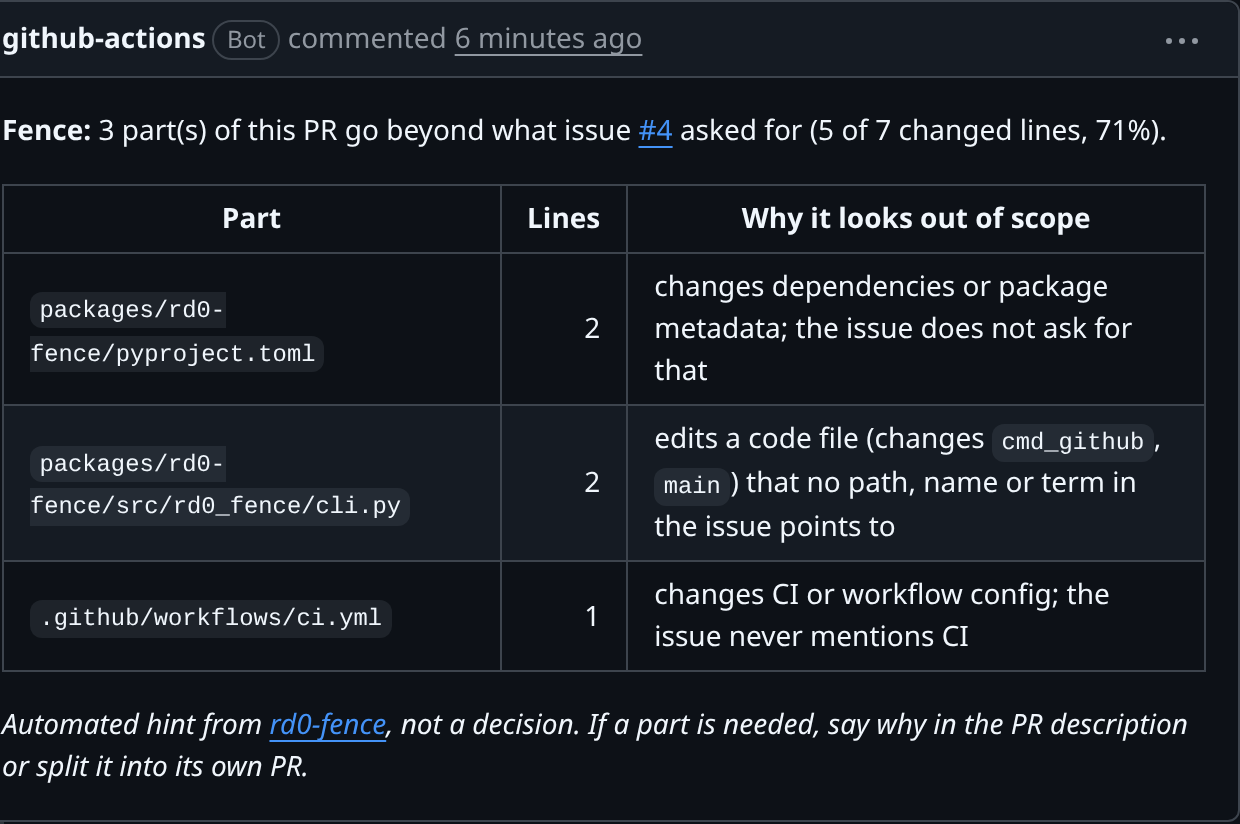
\includegraphics[width=\columnwidth]{fig_action_comment.png}
\caption{Fence's comment on a real PR: three changed files that issue~\#4 never asked for, each with a reason.}\label{fig:comment}\end{figure}

\section{Evaluation}
\textbf{Cost.} On \latN{} randomly drawn corpus PRs, one CPU process takes a median of \latMedian\,ms per PR (90th percentile \latPninety\,ms, 99th \latPnn\,ms), including parsing. The package has no runtime dependencies.

\textbf{Coverage.} On \nCorpus{} AIDev agent PRs with a linked issue, Fence could anchor \nAnchored{}; \nUnres{} (\pctUnres\%) were scope unresolvable. It flagged at least one part in \pctReach\% of anchored PRs. This is tool output, not a verified rate.

\textbf{Agreement with human labels.} On \nPai{} issue/patch pairs with PAIChecker's human scope-creep labels~\cite{wang2026paichecker}, Fence's reach has AUROC \aucFence{} against \aucSize{} for plain PR size, and adding Fence to size does not improve a cross-validated model (\cvSize{} to \cvSizeFence). The labels cover whole human-written patches rather than parts of agent PRs, but the result means a large PR is still the better single warning sign. Fence's value is different: it says \emph{which} part to look at and \emph{why}. Whether those part-level flags are right is what our \goldPRs-PR gold sheet will measure once it is labelled.

\textbf{Limitations.} Fence cannot see over-reach inside a file the issue names, and it flags support edits (an import, a fixture) that a reviewer would accept. Issues that point at nothing concrete get no code-level verdict.

\section{Availability}
Fence is MIT-licensed at \url{https://github.com/ReviewDebtZero/rd0-fence}, with the Action, the benchmark scripts, per-PR scores, the gold sheet and labeling app, and a demo video at \url{https://rd0-fence.netlify.app}.

\bibliographystyle{ACM-Reference-Format}
\bibliography{../refs}
\end{document}
